\documentclass[letterpaper,12pt,oneside]{article}\usepackage[]{graphicx}\usepackage[]{color}
%% maxwidth is the original width if it is less than linewidth
%% otherwise use linewidth (to make sure the graphics do not exceed the margin)
\makeatletter
\def\maxwidth{ %
  \ifdim\Gin@nat@width>\linewidth
    \linewidth
  \else
    \Gin@nat@width
  \fi
}
\makeatother

\definecolor{fgcolor}{rgb}{0.345, 0.345, 0.345}
\newcommand{\hlnum}[1]{\textcolor[rgb]{0.686,0.059,0.569}{#1}}%
\newcommand{\hlstr}[1]{\textcolor[rgb]{0.192,0.494,0.8}{#1}}%
\newcommand{\hlcom}[1]{\textcolor[rgb]{0.678,0.584,0.686}{\textit{#1}}}%
\newcommand{\hlopt}[1]{\textcolor[rgb]{0,0,0}{#1}}%
\newcommand{\hlstd}[1]{\textcolor[rgb]{0.345,0.345,0.345}{#1}}%
\newcommand{\hlkwa}[1]{\textcolor[rgb]{0.161,0.373,0.58}{\textbf{#1}}}%
\newcommand{\hlkwb}[1]{\textcolor[rgb]{0.69,0.353,0.396}{#1}}%
\newcommand{\hlkwc}[1]{\textcolor[rgb]{0.333,0.667,0.333}{#1}}%
\newcommand{\hlkwd}[1]{\textcolor[rgb]{0.737,0.353,0.396}{\textbf{#1}}}%

\usepackage{framed}
\makeatletter
\newenvironment{kframe}{%
 \def\at@end@of@kframe{}%
 \ifinner\ifhmode%
  \def\at@end@of@kframe{\end{minipage}}%
  \begin{minipage}{\columnwidth}%
 \fi\fi%
 \def\FrameCommand##1{\hskip\@totalleftmargin \hskip-\fboxsep
 \colorbox{shadecolor}{##1}\hskip-\fboxsep
     % There is no \\@totalrightmargin, so:
     \hskip-\linewidth \hskip-\@totalleftmargin \hskip\columnwidth}%
 \MakeFramed {\advance\hsize-\width
   \@totalleftmargin\z@ \linewidth\hsize
   \@setminipage}}%
 {\par\unskip\endMakeFramed%
 \at@end@of@kframe}
\makeatother

\definecolor{shadecolor}{rgb}{.97, .97, .97}
\definecolor{messagecolor}{rgb}{0, 0, 0}
\definecolor{warningcolor}{rgb}{1, 0, 1}
\definecolor{errorcolor}{rgb}{1, 0, 0}
\newenvironment{knitrout}{}{} % an empty environment to be redefined in TeX

\usepackage{alltt}
\usepackage[paperwidth=8.5in,paperheight=11in,top=1in,bottom=1in,left=1in,right=1in]{geometry}
\usepackage{setspace}
\usepackage[colorlinks=true,allcolors=Blue]{hyperref}
\usepackage[usenames,dvipsnames]{xcolor}
\usepackage{indentfirst}
\usepackage{titlesec}
\usepackage{multirow}
\usepackage{booktabs}
\usepackage{graphicx}
\usepackage{verbatim}
\usepackage{rotating}
\usepackage{tabularx}
\usepackage{outlines}
\usepackage{lineno}
\usepackage{array}
\usepackage{times}
\usepackage{cleveref}
\usepackage{acronym}
\usepackage[position=t]{subfig}
\usepackage{paralist}
\usepackage[noae]{Sweave}
\usepackage{natbib}
\usepackage{array}
\usepackage{pdflscape}
\usepackage{bm}
% \usepackage{showlabels}
\bibpunct{(}{)}{,}{a}{}{,}

% page margins and section title formatting
\linespread{2}
\setlength{\footskip}{0.5in}
\titleformat*{\section}{\Large\bf\em}
\titleformat*{\subsection}{\singlespace\large\bf}
\titleformat*{\subsubsection}{\singlespace\normalsize\bf\em}
\titlespacing{\section}{0in}{0in}{0in}
\titlespacing{\subsection}{0in}{0in}{0in}
\titlespacing{\subsubsection}{0in}{0in}{0in}

% cleveref options
\crefname{table}{Table}{Tables}
\crefname{figure}{Fig.}{Figs.}
\renewcommand{\figurename}{Fig.}

% aliased citations
\defcitealias{BeckIR}{Beck and Hagy, In review}
\defcitealias{CDMO14}{CDMO 2014}
\defcitealias{RDCT14}{RDCT 2014}

% acronyms
\acrodef{DO}[DO]{dissolved oxygen}
\acrodef{EPA}[EPA]{Environmental Protection Agency}
\acrodef{NERRS}[NERRS]{National Estuarine Research Reserve System}
\acrodef{RMSE}[RMSE]{root mean square error}
\acrodef{SWMP}[SWMP]{System Wide Monitoring Program}
\acrodef{WRTDS}[WRTDS]{weighted regression on time, discharge, and season}

% assorted functions
% for multiple rows in table headers
\newcommand{\head}[2]{\multicolumn{1}{>{\arraybackslash}p{#1}}{#2}}
% for milligrams per litre
\newcommand{\mgl}{mg L$^{-1}$}

% hides (not removes) numbering for section, subsection, etc.
% left indents
\renewcommand{\thesection}{}
\renewcommand{\thesubsection}{}
\renewcommand{\thesubsubsection}{}
\makeatletter
\def\@seccntformat#1{\csname #1ignore\expandafter\endcsname\csname the#1\endcsname\quad}
\let\sectionignore\@gobbletwo
\def\@subseccntformat#1{\csname #1ignore\expandafter\endcsname\csname the#1\endcsname\quad}
\let\subsectionignore\@gobbletwo
\def\@subsubseccntformat#1{\csname #1ignore\expandafter\endcsname\csname the#1\endcsname\quad}
\let\subsubsectionignore\@gobbletwo
\let\latex@numberline\numberline
\def\numberline#1{\if\relax#1\relax\else\latex@numberline{#1}\fi}
\makeatother

% dependent data



%knitr options


\IfFileExists{upquote.sty}{\usepackage{upquote}}{}
\begin{document}

\raggedbottom
\linenumbers
\raggedright
\urlstyle{same}
\setlength{\parindent}{0.5in}
\renewcommand\refname{References \vspace{12pt}}

%%%%%%
% title page
\begin{singlespace}
\title{{\bf {\Large Improving estimates of ecosystem metabolism by removing effects of tidal advection in dissolved oxygen time series}}}
\author{
  {\bf {\normalsize Marcus W. Beck$^1$, Michael C. Murrell$^2$, James D. Hagy III$^2$}}
  \\\\{\textit {\normalsize $^1$ORISE Research Participation Program}}
  \\{\textit {\normalsize USEPA National Health and Environmental Effects Research Laboratory}}
	\\{\textit {\normalsize Gulf Ecology Division, 1 Sabine Island Drive, Gulf Breeze, FL 32561}}
	\\{\textit {\normalsize Phone: 850-934-2480, Fax: 850-934-2401, Email: \href{mailto:beck.marcus@epa.gov}{beck.marcus@epa.gov}}}
  \\\\{\textit {\normalsize $^2$USEPA National Health and Environmental Effects Research Laboratory}}
	\\{\textit {\normalsize Gulf Ecology Division, 1 Sabine Island Drive, Gulf Breeze, FL 32561}}
	\\{\textit {\normalsize Phone: 850-934-2433, Fax: 850-934-2401, Email: \href{mailto:murrell.michael@epa.gov}{murrell.michael@epa.gov}}}
  \\\\{\textit {\normalsize $^3$USEPA National Health and Environmental Effects Research Laboratory}}
	\\{\textit {\normalsize Gulf Ecology Division, 1 Sabine Island Drive, Gulf Breeze, FL 32561}}
	\\{\textit {\normalsize Phone: 850-934-2455, Fax: 850-934-2401, Email: \href{mailto:hagy.jim@epa.gov}{hagy.jim@epa.gov}}}
	}
\date{}
\maketitle
\vfill{\centerline{\textit {\normalsize Running head: Improving Estimates of Estuary Metabolism}}}
\end{singlespace}
\clearpage

%%%%%%
% acknowledgments
\section{Acknowledgments}

We acknowledge the significant efforts of research staff and field crews from the \acl{SWMP} of the \acl{NERRS} for providing access to high quality data sets.  We thank Dr. Jane Caffrey for stimulating discussion and previous work on applications of the open-water method to estuarine monitoring data. This study was funded by the US \acl{EPA}, but the contents are solely the views of the authors.  Use of trade names does not constitute endorsement by the US government.

%%%%%%
% abstract
\newpage
\section{Abstract}
Reliable estimates of ecosystem metabolism depend on measures of \ac{DO} flux that are dominated by biological processes.  Long-term time series of \ac{DO} measurements may include variation related to both biological and physical processses such that the use of observed data may be insufficient or even misleading in some examples.  Statistical modelling techniques that dynamically quantify variation in \ac{DO} over time and tidal changes have the potential to isolate biological signals in \ac{DO} variation to more accurately estimate metabolism.  A weighted regression method that estimates \ac{DO} as a function of time and tidal height was developed to normalize, or detide, the predicted \ac{DO} signal to remove the influence of physical advection on metabolism estimates.  First, a simulation approach was used to create multiple \ac{DO} time series with known additive components of biological and physical variation on different periods.  Comparisons of detided estimates with the known, simulated biological component of the \ac{DO} signal suggested the method accurately and precisely removed varation attributed to tidal advection.  Extension of the method to four case studies provided a proof of concept illustrating the method could be useful for real-world applications. We provide a detailed discussion on use of the method for improving certainty in evaluation of \ac{DO} measurements from sites with strong tidal influences.  Moreover, we propose that the method could expand use of the open-water method for estimating ecosystem metaoblism in estuaries given that the approach can produce robust estimates of \ac{DO} values that are independent of tidal advection.  In particular, this could facilitate the use of shorter deployment periods for water quality monitors or incomplete time series given that known biases related to water movement could be removed with weighted regression. 

\acresetall
\clearpage

%%%%%%
% intro
\section{Introduction} \label{intro}

Time series of dissolved oxygen are increasingly used to estimate ecosystem metabolism \citep{Kemp12,Needoba12}.  Integrated measures of metabolism describe the balance between production and respiration processes that create and consume organic matter, respectively.  Although metabolic rates vary naturally between systems \citep{Ziegler98,Caffrey04,Russell07}, anthropogenic nutrient sources are often contributing factors that increase rates of production \citep{Diaz08}.  Inputs of limiting nutrients beyond background concentrations may decrease the resilience of an ecosystem such that higher rates of production are coupled with higher biological oxygen demand \citep{Yin04,Kemp09}.  Cultural eutrophication is frequently linked to declines in water quality through lower levels of dissolved oxygen, degradation in aquatic vegetation habitat, and increased frequency of harmful algal blooms \citep{Cloern96,Short96,Rabalais02}.  Reliables estimates of ecosystem metabolism are critical for measuring both background rates of production and potential impacts of human activities on ecosytem condition.     

Ecosystem metabolism can be estimated using two basic techniques, each of which is appropriate under different conditions or assumptions \citep{Kemp12}.   Bottle-based techniques rely on rate measurements from discrete water quality samples, whereas open-water techniques infer metabolic rates using \textit{in situ} measurements from continuous monitoring data.  Bottle-based techniques partition metabolic contributions into discrete habitats, such as pelagic production rates during specific time periods \citep{Kemp12}.  However, such measurements cannot estimate whole ecosystem metabolism if significant metabolism occurs in habitats that are not sampled, such as the benthos.  As such, open-water metabolism provides an integrative measure of process rates from \textit{in situ}, continuous monitoring data.  Originally conceived for streams \citep{Odum56}, the open-water method has been used with varying success in lakes \citep{Staehr10,Coloso11,Batt12} and estuaries \citep{Caffrey04,Hopkinson05,Caffrey13}.  As with any method, the ability to accurately estimate whole system metabolism depends on the degree to which assumptions of the theory are met.  Such assumptions are often only implicity verified in practice, leading to potential biases.

The open-water method uses the diel fluctuation of dissolved oxygen to infer rates of ecosytem metabolism, after correcting for air-water gas exchange \citep{Kemp12}.  Daily integrated measurements of metabolism represent the balance between daytime production and nighttime respiration.  The fundamental assumption is that the time series of \ac{DO} describes the same water mass over time \citep{Needoba12}.  Estimates of metabolism from a single location may be inaccurate if substantial variation in water column mixing occurs throughout the period of observation \citep{Russell07}.  Application to lakes or estuaries have often assumed that a single sampling station provides sufficient data for estimating metabolism \cite{Staehr10}.  While single stations may be valid under specific conditions, numerous studies have shown that the open-water method may be inappropriate given the effects of physical mixing in lakes or estuaries \citep{Ziegler98,Caffrey03,Coloso11,Batt12,Nidzieko14}.  An extensive analysis by \citet{Caffrey03} applied the open-water method to estimate metabolim at 28 continuous monitoring stations at 14 US estuaries.  A significant portion of the estimates were negative for production and positive for respiration, i.e., opposite in sign given the assumptions of the method.  These `anamolous' values were attributed to the effects of tidal advection such that water masses with different metabolic histories were sampled at multiple sites.  Moreover, anomalous estimates were included in annual averages of ecosystem metabolism such that inferred rates could have been biased.

The effects of tidal advection on estimates of ecosystem metabolism have been emphasized in numerous studies \citep{Ziegler98,Collins13,Howarth14,Nidzieko14}, although systematic estimates of its effects have been minimal.  Analytical techniques to evaluate and correct for tidal advection could improve certainty in metabolism estimates and increase the use of data from shorter deployment periods if sources of bias are removed.  This article describes the application of a method for filtering an observed \ac{DO} time series for estimated tidal effects to more accurately quantify estimates of ecosystem metabolim for estuaries.  Specifically, the effects of tidal advection on \ac{DO} observations are removed to improve estimates of open-water metabolism with continuous water quality data.  We use a weighted regression approach developed to resolve trends in pollutant concentrations in streams and rivers \citep{Hirsch10}.  The weighted regression approach creates dynamic predictions of \ac{DO} as a function of time and tidal height change, which are then used to filter, or detide, the \ac{DO} signal.  First, we use a simulation approach to create time series of \ac{DO} observations with known characteristics to evaluate ability of the weighted regression to remove the effects of tidal advection.  Second, four case studies were chosen from the \aclu{NERRS} (\acs{NERRS}, \citealt{Wenner04}) to illustrate the method for adjusting estimates of ecosystem metabolism.  Overall, the analysis is meant to better characterize the relative roles of biological and physical processes in estuarine systems.

%%%%%%
% materials and procedures
\section{Materials and Procedures}

\subsection{Weighted regression for modelling and detiding \ac{DO} time series}

The weighted regression model for filtering \ac{DO} time series for tidal effects was adapted from the \ac{WRTDS} method \citep{Hirsch10}.  The functional form of the model is a simple linear regression:
\begin{equation}\label{funform}
DO_{obs}= \beta_0 + \beta_1 t + \beta_2 H
\end{equation}
where observed \ac{DO} is a linear function of time $t$ and tidal height $H$.  Time is a continuous variable for the day and time of each obervation with time as a proportion of the number of total observations added to each day.  The beginning of each day was considered the nearest thirty minute observation to sunrise for the location.  Our model also differed from the original \ac{WRTDS} method that included parameters to estimate variation of the response variable on a sinuisoidal period.  \ac{DO} variation was not modeled using this approach to avoid constraining parameter estimates by periodic components.

Weighted regression was implemented as a moving window that allowed for estimation of \ac{DO} throughout the time series by adapting to variation through time as a function of tide. Regression models were estimated sequentially for each observation in the time series using dynamic weight vectors that change with the center of the window.  Weight vectors quantified the relevance of observations to the center of the window in respect to time, hour of the day, and tidal height.  Specifically, weights were assigned to each variable using a tri-cube weighting function \citep{Tukey77,Hirsch10}:
\begin{equation}
w= \left\{ 
  \begin{array}{l l}
    \left(1-\left(d/h\right)^3\right)^3 & \quad \textrm{if } |d| \leq h \\
    0 & \quad \textrm{if } |d| > h 
  \end{array} \right.
\end{equation}
where the weight $w$ of each observation is inversely proportional to the distance $d$ from the center of the window such that observations more similar to the point of reference are given higher importance in the regression.  Weights exceeding the maximum width of the window $h$ are equal to zero.  The tri-cube weighting function is similar to a Gaussian distribution such that weights decrease gradually from the center until the maximum window width is reached.  Regressions that use simpler windows (e.g., boxcar approach) are  more sensitive to influential observations as they enter or leave the window, whereas the tri-cube function minimizes their effect through gradual weighting of observations from the center \citep{Hirsch10}.  The final weight vector for each observation is the product of three separate weight vectors for decimal time (day), hour, and tidal height. Windows for time and hour weight observations based on distance (time) from the center of the window.  The window for tidal height weights observations based on the difference from the center as a proportion of the total tidal height range.  For example, a half-window width of 0.5 means that observations are weighted proportionately within +/- 50\% the total range referenced to the tidal height in the center of the window. A low weight is given to an observation if any of the three weighting values were not similar to the center of the window since the final weight vector is the product of three weight vectors for each variable (see the link in the \hyperref[multi]{multimedia} section for graphical display of different weights).    

The choice of window widths for weight vectors strongly affects the model results.  Excessively large or small window widths may respectively under- or over-fit the observed data.  Accordingly, appropriate window widths depend on the objective for using the model.  The weighted regression approach can be used for both predicting observed \ac{DO} and filtering the observed time series to remove the variance that coincided with the tidal cycle.  Window widths that minimize prediction error or fit to the observed data are typically smaller than the widths for filtering the time series.  Similarly, window widths that more effectively detide the \ac{DO} signal may produce imprecise predictions for the observed data.  Evaluations of the weighted regression method with simulated \ac{DO} time series, described below, used multiple window widths to evaluate the ability of the model to filter the \ac{DO} signal.  The ability to predict observed \ac{DO} was not a primary objective such that the window widths were evaluated only in the context of removing tidal variation from the \ac{DO} time series.  

The normalization approach to filter tidal variation from the observed \ac{DO} time series differs slightly from methods in \citet{Hirsch10}.  The previous approach used a two-dimensional grid predicted for stream pollutant concentrations across the time series and the range of discharge values observed in the study system \citep{Hirsch10}.  Normalized or discharge-independent values for pollutant concentration were obtained by averaging grid predictions across the discharge values that were likely to occur on a given day.  Rather than creating a two-dimensional grid of \ac{DO} related to time and tidal height change, the normalized time series herein were the model predictions conditional on time and constant tidal height set to the mean:
\begin{equation} \label{do_nrm}
DO_{nrm} = f(DO_{obs}|\bar{H}, t)
\end{equation}
such that the normalized time series represents \ac{DO} variation related to biological processes (\cref{fig:do_dtd}).   

%%%%%%
% assessment
\section{Assessment}

\subsection{Simulation of \ac{DO} time series}

To test the ability of the weighted regression to filter the \ac{DO} signal for apparent tide effects, multiple time series with known characteristics were simulated and filtered.  Observed \ac{DO} time series were simulated as the sum of variation from biological processes and physical effects related to tidal advection:  
\begin{equation} \label{do_obs}
DO_{obs} = DO_{bio} + DO_{adv}
\end{equation}
Biological \ac{DO} signals are inherently noisy \citep{Batt12} and variance can be further described as:
\begin{equation} \label{do_bio} 
DO_{bio} = DO_{die} + DO_{unc}
\end{equation} 
\begin{equation} \label{do_unc}
DO_{unc} = \epsilon_{obs} + \epsilon_{proc}
\end{equation}
where the biological \ac{DO} signal is the sum of diel variation plus uncertainty or noise.  Total uncertainty in the biological \ac{DO} signal is described as variation from observation and process uncertainty \citep{Hilborn97}.  Multiple time series at 30 minute time steps over 30 days were created by varying the relative magnitudes of each of the four components of observed \ac{DO} in \cref{do_obs,do_bio,do_unc} to test the effectiveness of weighted regression under different scenarios.  Accordingly, observed \ac{DO} was generalized as the additive combination of four time series (\cref{fig:do_sim}):
\begin{equation} \label{do_obs_all}
DO_{obs} = DO_{adv} + DO_{die} + \epsilon_{obs} + \epsilon_{pro}
\end{equation} 

Each component of the simulated time series was created as follows.  First, the diel component, $DO_{die}$, was estimated using a sine/cosine function \citep{Cryer08}:
\begin{equation} \label{do_sin}
DO_{die} = \alpha + \beta\cos\left(2\pi ft + \Phi\right)
\end{equation}
such that the mean DO $\alpha$ was 8, amplitude $\beta$ was 1, $f$ was 1/48 to repeat on a 24 hour period every 30 minutes, $t$ was the time series vector and $\Phi$ was the x-axis origin set for an arbitrary sunrise at 630am.  The diel signal was increasing during the day and decreasing during the night for each 24 hour period and ranged from 7 to 9 mg L$^{-1}$.  Noise or uncertainty was added to the diel \ac{DO} signal to simulate natural variation in \ac{DO} throughout the time series (\cref{fig:do_sim}).  Total uncertainty was the sum of observation and process uncertainty for $n = 1440$ (30 minutes by 30 days) observations \citep{Hilborn97}, such that:
\begin{equation} \label{do_unc_n}
DO_{unc, n} = \epsilon_{obs, n} + \int_{t = 1}^{n} \epsilon_{pro, t}
\end{equation}
where observation and process uncertainty ($\epsilon_{obs}$, $\epsilon_{pro}$) were simulated as normally distributed random variables with mean zero and standard deviation varying from zero to an upper limit, described below.  To induce auto-correlation, process uncertainty was estimated as the cumulative sum of $n$ observations where the noise at time $t+1$ was equal to the noise at time $t$ plus additional variation drawn from the normal distribution.  The noise vector for process uncertainty was rescaled to constrain the variation within the bounds for standard deviation defined by the random variable. The total uncertainty, $DO_{unc}$, was added to the diel \ac{DO} time series to create the biological \ac{DO} time series (\cref{do_bio,fig:do_sim}).

A semidiurnal tidal series was simulated as a sine wave with a period of 12.5 hours to represent the principal lunar component \citep{Foreman89}.  The amplitude was set to 1 meter and centered  at 4 meters.  Initial assessments indicated that tide type (i.e., diurnal, semidiurnal, mixed) did not signifcantly affect the outcome of the results and a semidiurnal time series was used to reduce the total number of simulations.  The tidal time series was added to the biological \ac{DO} series to simulate \ac{DO} changes with advection, $DO_{adv}$ (\cref{do_obs_all,fig:do_sim}). Conceptually, this vector represents the rate of change in \ac{DO} as a function of horizontal water movement from tidal advection such that:
\begin{equation} \label{deltdo}
\frac{\delta DO_{adv}}{\delta t} = \frac{\delta DO}{\delta x} \cdot \frac{\delta x}{\delta t}
\end{equation}
\begin{equation} \label{deltx}
\frac{\delta x}{\delta t} = k \cdot \frac{\delta H}{\delta t}
\end{equation}
where the first derivative of the tidal time series, as change in height over time $\delta H / \delta t$, is multiplied by a constant $k$, to estimate horizontal tidal excursion over time, $\delta x / \delta t$.  The horizontal excursion is assumed to be associated with a horizontal \ac{DO} change, $\delta DO / \delta x$, such that the product of the two estimates the \ac{DO} change at each time step from advection, $DO_{adv}$. In practice, the simulated tidal signal was used to estimate $DO_{adv}$:
\begin{equation} \label{do_advp}
DO_{adv} \propto H
\end{equation}
\begin{equation} \label{do_adv}
DO_{adv} = 2\cdot a + a \cdot \frac{H- \min H}{\max H - \min H}
\end{equation}
where $a$ is analogous to $k$ in \cref{deltx} and is chosen as the transformation parameter to standardize change in \ac{DO} from tidal height change to desired units.  For example, $a = 1$ will convert $H$ to a scale that simulates changes in \ac{DO} from tidal advection that range from +/- 1 mg L$^{-1}$.  The final time series for observed \ac{DO} was the sum of biological \ac{DO} and advection \ac{DO} (\cref{do_obs,fig:do_sim}).

\subsection{Evaluation of weighted regression with simulated \ac{DO} time series}

Multiple time series were simulated by varying the conditions in \cref{do_obs,do_bio,do_unc,do_obs_all,do_sin,do_unc_n,deltdo,deltx,do_advp,do_adv}. Specifically, the simulated data varied in the relative amount of noise in the measurement ($e_{pro}$, $e_{obs}$), relative amplitude of the diel \ac{DO} component ($DO_{die}$), and degree of association of the tide with the \ac{DO} signal ($DO_{adv}$).  Three levels were evaluated for each variable: relative noise as 0, 1, and 2 standard deviations for both process and observation uncertainty, amplitude of diel biological \ac{DO} as 0, 1, and 2 mg L$^{-1}$, and \ac{DO} change from tidal advection as 0, 1, and 2 mg L$^{-1}$. A total of 81 time series were created based on the unique combinations of parameters (\cref{fig:sim_ex}).  Three half window widths for each variable (day, hour of day, and tide height) were evaluated for each simulation: decimal time as 1, 3, and 6 days, time of day as 1, 3, and 6 hours, and tidal height as 0.25, 0.5, and 1 as a proportion of the total range given the height at the center of the window.  The window widths were chosen based on preliminary assessments that suggested variation in model performance was adequately captured by these values.  In total, 27 window width combinations were evaluated for each of 81 simulated time series, producing results for 2187 weighted regressions.

The detided or normalized values for each regression were compared to the simulated data to evaluate the ability of weighted regression to reproduce the biological \ac{DO} signals. Results were summarized using Pearson correlation coefficients and the \ac{RMSE} between the detided time series and the biological \ac{DO} time series as a known component of the observed.  Overall, the weighted regressions provided accurate results for the detided time series compared to the `true' biological time series regardless of the simulation parameters (\cref{tab:dtd_perf1}) or window widths (\cref{tab:dtd_perf2},   results for each simulation can be viewed using the link in the \hyperref[multi]{multimedia} section).  Mean correlation for all time series and window widths between the detided and biological values was 0.60, with values ranging from -0.78 to 1.00.  Mean error was 1.21, with values ranging from 0 to 2.40.  Simulations with very poor performance (e.g., negative correlations) were those that had minimum widths for day windows and maximum widths for hour windows, or were those with the \ac{DO} signal composed entirely of noise from observation uncertainty. Conversely, simulations with detided time series that were identical to the true time series (e.g., correlation of one, \ac{RMSE} of zero) were those for which there was no biological or tidal influence.  Although these examples do not represent real-world scenarios, they were included in the simulations to provide verification that the weighted regression provided reasonable results given extremes.  

Characteristics of \ac{DO} time series that contributed to improved model performance were increasing amplitude of the diel \ac{DO} component ($DO_{die}$) and increasing process uncertainty ($e_{pro}$), whereas increasing observation uncertainty contributed to decreased performance (\cref{tab:dtd_perf1,fig:err_surf1}).  Model performance was minimally influenced by magnitude of the tidal advection component ($DO_{adv}$), although performance decreased slightly with increasing tidal effects.  Increasing widths for day and tidal proportion windows contributed to increasing model performance, whereas the opposite was true for increasing hour windows (\cref{tab:dtd_perf2,fig:err_surf2}).  Graphical summaries of model performance by simulation parameters (\cref{fig:err_surf1}) and half window widths (\cref{fig:err_surf2}) support the general trends described by \cref{tab:dtd_perf1,tab:dtd_perf2}.

\subsection{Validation of weighted regression with case studies}

\ac{NERRS} is a federally-funded network of 28 protected estuaries established for long-term research, water-quality monitoring, education, and coastal stewardship \citep{Wenner04}.  Continuous water quality data have been collected at \ac{NERRS} sites since 1994 through the \ac{SWMP}.  In addition to providing a basis for trend evaluation, data from \ac{SWMP} provides an ideal opportunity to evaluate long-term variation in water quality parameters from biological and physical processes.  Continuous \ac{SWMP} data can be used to describe \ac{DO} variation at sites with different characteristics, including variation from ranges in tidal regime \citep{Sanger02} and rates of ecosystem production \citep{Caffrey03,Caffrey04}.  

Continuous \ac{DO} time series and tidal height measurements at four sites from the \ac{SWMP} database \citepalias{CDMO14} were used to validate the detiding model with real data.  Monitoring data from January 1\textsuperscript{st} to December 31\textsuperscript{st} 2012 were obtained from a range of geographic locations (\cref{fig:case_map,tab:case_att}). Astronomical tidal heights were predicted for each site using harmonic regression applied to the sonde depth data (\texttt{oce} package in R, \citealt{Foreman89}, \citetalias{RDCT14}). Although, the depth data represent tidal height variation from both astronomical (i.e., gravitational effects) and meteorological (e.g., wind, precipitation inflows) sources, we isolated the former given that daily metabolism estimates were more likely to be affected by repeated diel cycling from normal tidal changes.  Each station was also chosen based on highly significant correlations between \ac{DO} and tidal changes.  The four sites included the Vierra Mouth station at Elkhorn Slough (California, 36.81$^{\circ}$N, 121.78$^{\circ}$W), Bayview Channel at Padilla Bay (Washington, 48.50$^{\circ}$N 122.50$^{\circ}$W), Middle Blackwater River station at Rookery Bay (Florida, 25.93$^{\circ}$N 81.60$^{\circ}$W), and Dean Creek station at Sapelo Island (Georgia, 31.39$^{\circ}$N 81.28$^{\circ}$W).  The stations are generally macrotidal semidiurnal or mixed semidiurnal and net heterotrophic on an annual basis (\cref{tab:case_att}).  Net heterotrophy (i.e., respiration exceeding production) is typical for shallow water systems at temperate latitudes \citep{Caffrey03}, although values in \cref{tab:case_att} are from observed \ac{DO} time series that are strongly influenced by tidal advection.

\subsection{Estimates of ecosystem metabolism before and after detiding} \label{met_sec}

The weighted regression method was applied to the time series for each station to obtain a detided \ac{DO} time series for estimating metabolism.  Half window widths of six days, one hour, and a tidal proportion of one half were chosen based on a balance between large and small window widths, although the chosen window widths are arbitrary and a more exhaustive evaluation should be conducted prior to using the results to inform management. Unlike the simulated data, the true biological \ac{DO} signal was unknown for the case studies.  Accordingly, results were evaluated  using correlations of \ac{DO} and metabolism estimates with tidal height before and after application of the model.  Daily metabolism estimates before and after detiding were compared to the mean rate of tidal height change (i.e., first derivative of the predicted tidal height) for each day during separate solar periods.  Production rates were compared to mean rates of tidal height change during the day, respiration rates were compared to mean rates of change during the night, and net metabolism rates were compared to mean rates of change for the total 24 hour period each day.  Results were also evaluated based on the occurrence of `anomalous' daily production or respiration estimates, where anomalous was defined as negative production during the day and positive respiration estimates during the night.  Anomalous values have been previously attributed to the effects of physical processes on \ac{DO} time series \citep{Caffrey03}.  We hypothesized that metabolism esimates using the detided signal would contain less `anomalous' values than those from the observed \ac{DO} time series.  Although anomalies could be caused by processes other than tidal advection, e.g., abiotic dark oxygen production \citep{Pamatmat97}, we assume that physical processes are the dominant sources of these values given the tidal characteristics at each site.  Finally, means and standard errors of metabolism estimates were evaluated before and after detiding to determine if annual aggregations were significantly different.   

Ecosystem metabolism was estimated from the \ac{DO} time series using the open-water technique \citep{Odum56} as described in \citet{Caffrey13}.  The method is used to infer net ecosystem metabolism using the mass balance equation:
\begin{equation} \label{metrate}
\frac{\delta DO}{\delta t} = P - R + D
\end{equation}
where the change in \ac{DO} concentration ($\delta DO$, g O$_2$ m$^{-3}$) over time ($\delta t$, hours) is equal to photosynthetic rate ($P$, g O$_2$ m$^{-3}$ hr$^{-1}$) minus respiration rate ($R$, g O$_2$ m$^{-3}$ hr$^{-1}$), corrected for air-sea gas exchange at the surface ($D$, g O$_2$ m$^{-3}$ hr$^{-1}$) \citep{Caffrey13}. $D$ is estimated as the difference between the \ac{DO} saturation concentration and observed \ac{DO}, multiplied by a volumetric reaeration coefficient, $k_a$ \citep{Thebault08}.  The diffusion-corrected \ac{DO} flux estimates were averaged during day and night for each 24 hour period in the time series, where flux is an hourly rate of \ac{DO} change as the difference between observations at time $t$ and $t+1$ on an hourly scale.  Areal respiration rates were assumed constant during the night and substracted from daily gross production estimates to yield net ecosystem metabolism (\cref{tab:case_att}).  

Detiding had significant effects on the correlations between tidal height changes, \ac{DO} time series, and metabolism estimates (\cref{tab:cor_res},  see the link in the \hyperref[multi]{multimedia} section for graphical results of each case study).  Correlations of observed \ac{DO} time series with predicted tidal height were highly significant, with all sites indicating positive relationships, except Padilla Bay where tidal increases were associated with declines in \ac{DO}  concentration.  This suggests that seaward water masses were less anoxic than landward masses, with the opposite being true for Padilla Bay. The detided \ac{DO} time series had greatly reduced correlations with tidal height, although relationships were still significant after detiding likely because of the large sample size for each site (n $\approx$ 17500). Comparison of metabolic rates to tidal changes before and after detiding produced inconsistent results (\cref{tab:cor_res}).  Correlations for Elkhorn Slough and Sapelo Island showed consistent reductions in all three metabolims estimates after detiding.  Correlations for Padilla Bay and Rookery Bay were of opposite sign and greater magnitude after detiding for production and respiration, although net metabolism estimates had reduced correlations.  

The proportion of daily integrated metabolism estimates that were anomalous (negative production, positive respiration) were significantly reduced for most sites after detiding (\cref{tab:case_res}).  Before detiding, anomalous values ranged from 0.09 (Rookery Bay) to 0.22 (Padilla Bay) for production and 0.08 (Rookery Bay) to 0.21 (Elkhorn Slough) for respiration. Anomalous values were reduced to near zero for Rookery Bay and Sapelo Island, by approximately half for Padilla Bay (0.13 for production, 0.13 for respiration), and only slightly reduced for Elkhorn Slough (0.17 for production, 0.17 for respiration).  Metabolism estimates using detided \ac{DO} time series had decreased mean production and respiration for Elkhorn Slough, increased mean production and respiration for Padilla Bay, and generally unchanged mean production and respiration for Rookery Bay and Sapelo Island (\cref{tab:case_res}).  Mean net ecosystem metabolism was unchanged for all sites.  Decreases in the standard erorr for all metabolism estimates (production, respiration, and net) were observed for all cases after detiding.  

An example from Sapelo Island illustrates the effects of weighted regression on \ac{DO} and metabolism estimates (\cref{fig:phase_out,fig:phase_in,fig:case_ex}).   A two-week period in February shows when the tidal changes were both in and out of phase with the diel cycling.  Maximum tide heights were generally out of phase with the diel cycle during the first week such that low tides were observed during the middle of the night and the middle of the day (\cref{fig:phase_in}).  The opposite scenario occurred during the second week when the maximum tide height occured during the day and night (\cref{fig:phase_in}).  The effects of tidal height change on the observed \ac{DO} time series are visually apparent in the plots. The first week illustrates a strong negative bias (less respiration, less production) in the observed \ac{DO} signal from low tides at mid-day and mid-night, whereas the second example illustrates a strong positive bias (more respiration, more production) in the observed \ac{DO} from high tides. These biases are apparent in the metabolism estimates using the observed data (\cref{fig:case_ex}).  Anomalous estimates occur when low tides are in phase with the solar cycle, whereas metabolism estimates are likely over-estimated when high tides are in phase with the solar cycle.  The detided time series shows noticeable changes given the direction of bias from the phasing between tidal height and diel period.  \ac{DO} values were higher after detiding when low tides occurred during night and day periods, whereas \ac{DO} values were lower after detiding when high tides occurred during day and night periods (\cref{fig:phase_out,fig:phase_in}).  Changes in metabolism estimates after detiding were also apparent, such that the anomalous values were removed during the first week and the positive bias in the second week is decreased.  Detiding had similar effects for the remaining sites, particularly when tidal changes were strongly in or out of phase with diel periods. 

\subsection{Effects of aggregation and importance of detiding}

A final point of concern is the period of observation within which observed \ac{DO} is affected by tidal height changes and the extent to which this affects the interpretation of ecosystem metabolism.  From a management or ecological perspective, the effects of tidal variation on daily estimates may not be a primary concern given that seasonal or annual rates may be more relevant for evaluating ecosystem dynamics with continuous monitoring data.  The example from Sapelo Island in the previous section highlights this point given that mean production and respiration estimates before and after detiding were generally unchanged for the two-week period. \cref{tab:case_res} also indicated that mean annual estimates of production and respiration were unchanged for Rookery Bay and Sapelo Island, whereas production and respiration estimates were significantly different for Elkhorn Slough and Padilla Bay. Although we acknowledge that the specific results may be related to the window widths, this suggests that tidal effects contribute to changes in metabolic estimates from observed time series that are aggregated on longer time periods.  Therefore, an evaluation of the effects of tidal variation on ecosystem metabolism for different periods of observation is critical for understanding practical implications of weighted regression.  Specifically, when should detiding be applied if aggregation of observed data on longer time periods removes potential bias?  A comparison of observed and detided estimates that are aggregated over different periods of observation (e.g., annual, seasonal, monthly) could help address this question.

The observed and detided daily estimates were averaged by month and season (Fall, Spring, Summer, and Winter) for each case study to evaluate effects of aggregation on mean production and respiration estimates.  Mean annual estimates in \cref{tab:case_res} also provided a basis of comparison with monthly and seasonal aggregation. Significant variation in aggregated production and respiration estimates for month and season was observed for each case study (\cref{fig:metab_sum1,fig:metab_sum2}).  Detided production and respiration estimates for Padilla Bay and Rookery Bay exhibited seasonal and monthly variation that was more characteristic of expected trends with increases in metabolism during warmer months.  Specifically, production estimates based on observed \ac{DO} were substantially muted for both Padilla Bay (\cref{fig:metab_sum1}) and Rookery Bay (\cref{fig:metab_sum2}) during summer months, whereas values were significantly higher based on the detided data. Results for Sapelo Island suggested that winter and summer months were under- and over-estimated, respectively, based on the observed data.  Results for Elkhorn Slough varied significantly such that production and respiration were significantly reduced after detiding regardless of the aggregation period.  Overall, these trends emphasize the importance of considering different aggregation periods for interpreting metabolism estimates.  Each case study showed differences in observed and detided values at monthly and seasonal aggregations, whereas only two of the four case studies had mean aggregated estimates that were substantially different (Elkhorn Slough and Padilla Bay, \cref{tab:case_res}).  Periods of observation as long as one year may include significant sources of bias from tidal advection, suggesting the need for applying weighted regression given careful consideration of appropriate window widths.       

 

%%%%%%
% discussion
\section{Discussion}

The primary objective for development and application of the weighted regression technique was to provide a method for more accurately estimating ecosystem metabolism by removing variation associated with tidal change in observed \ac{DO} time series.  The application of weighted regression to simulated \ac{DO} time series with known characteristics and extension to continuous monitoring data from selected \ac{NERRS} sites provided a proof-of-concept that the method can isolate and remove variation in observed \ac{DO} from tidal change.  Further, aggregation of metabolism estimates using the detided \ac{DO} time series were significantly different than those using the observed data, particularly for relatively long periods of observation. These results suggest that previous estimates of annual means may not accurately reflect true metabolic signals if the effects of tidal variation confound biological signals in observed \ac{DO} time series.  Additionally, variation of aggregated metabolism estimates were substantially reduced after detiding, suggesting greater confidence in interpreting detided estimates even if the mean values are similar.  Monitoring data for periods of observation up to one year may also produce significantly different metabolism estimates if observed data are not detided. 

Comparisons between detided and biological \ac{DO} time series from the simulations indicated that adequate results can be obtained from weighted regressions for a range of characteristics of \ac{DO} time series.  An examination of scenarios that produced abnormal results can provide additional insight into factors that affect the performance of weighted regression.  For example, poor performance was observed when the observation uncertainty ($\epsilon_{obs}$) was high and both process uncertainty ($\epsilon_{pro}$) and tidal advection ($DO_{adv}$) were low.  These examples represent time series with excessive random variation, no auto-correlation, and no tidal influence.  Poor performance is expected because the weighted regression models a non-existent tidal signal in a very noisy \ac{DO} time series.  These results were observed even for time series with a large diel component of the biological \ac{DO} signal, suggesting that the model will produce random results in microtidal systems with high noise and no serial correlation.  From a practical perspective, weighted regression should not be applied to noisy time series if there is not sufficient evidence to suggest the variation is related to tidal changes.  Similarly, results with perfect or near-perfect correlations between detided and biological \ac{DO} time series were observed when observation uncertainy and tidal effects were not components of the simulated time series.  Although there is no logical basis for applying weighted regression to time series with no apparent tidal influences, the results will be as expected, as was true for cases with low tidal advection, high observation uncertainty, and low process uncertainty.  We emphasize that the weighted regression should only be applied to time series for which specific conditions apply, as described below.  

The performance metrics used to evaluate weighted regression with the case studies suggested that detiding provided more accuate estimates of ecosystem metabolism.  Correlations of metabolism estimates with tidal height changes after detiding were generally reduced, although trends were not always consistent as correlations were reduced in some cases (Sapelo Island) or reversed in others (Padilla Bay).  However, correlations of net metabolism estimates were reduced in all cases.  Tidal height change provided a proxy for horizontal advection that directly affects the measured rate of change of oxygen.  Further, changes in \ac{DO} concentration represent integrated measures of both production and respiration (\cref{metrate}).  The inconsistent results in \cref{tab:cor_res} are potentially related to the effects of horizontal advection on the integrated \ac{DO} signal, given that production and respiration each represent a unique component of the diel \ac{DO} variation that is directly affected by tidal variation.  Regardless, the proportion of anomalous metabolism estimates was reduced by detiding for all case studies, although this measure may also be an incomplete indication of the combined effects of tidal variation.  Negative production and positive respiration estimates suggest assumptions of the open-water method are violated \citep{Needoba12}, whereas `normal' estimates (positive production and negative respiration) may still include a significant source of bias from physical advection by providing over-estimates of true values.  For example, \citet{Nidzieko14} observed that net metabolism at Elkhorn Slough was more often heterotrophic during maximum spring tides that occurred at nighttime, as a substantially larger area of salt marsh was inundated leading to higher respiration estimates.  Although this result supports our general conclusions, a broader discussion regarding whether or not this represents an actual bias in metabolism from physical advection may be needed. 

A strength of the weighted regression approach is a lack of assumptions describing the relationships between \ac{DO} and tidal variation over time.  Although the functional form of the model is a simple linear regression with only two explanatory variables (\cref{funform}), the moving window approach combined with the adaptive weighting scheme allows for quantification of complex tidal effects that may not be possible using alternative approaches.  For example, \citet{Batt12} described the use of a moving window or Kalman filter \citep{Harvey89} to improve estimates of ecosystem metabolism in lakes.  The approach minimizes the influences of process and observation uncertainty on observed \ac{DO} time series, which is attributed to the effects of water movement on metabolic signals.  Although a similar approach may be useful for estuaries if process and observation uncertainty are the only sources of variation in the \ac{DO} series, the weighted regression approach is more appropriate if periodic tidal advection is the primary confounding factor.  Additionally, results from the case studies illustrated the ability of the weighted regression approach to model changes over time in the relationships between tidal change and \ac{DO}.  Results for Padilla Bay and Rookery Bay suggested that detiding had the largest effect during the summer, whereas the results for cooler months were not significantly different from the observed.  The weighted regression method produced detided time series that accommodated seasonal variation in \ac{DO} conditional on tidal height change, whereas moving window filters or standard regression techniques would likely not have characterized these dynamic relationships.

%%%%%%
% comments and recs
\section{Comments and recommendations}

Results from the simulations and case studies suggested that weighted regression can be a practical approach for detiding \ac{DO} time series to remove the effects of physical advection on estimates of ecosystem metabolism.  However, application of the method may only be appropriate under specific situations.  The case studies were chosen based on the relatively high proportion of metabolism estimates that were anomalous and the strength of correlation between the observed \ac{DO} time series and tidal height.  Despite these similarites among the case studies, detiding had variable effects on metabolism estimates.  The results for Elkhorn Slough and Padilla Bay are of particular concern given that mean annual estimates were substantially different compared to those from the observed \ac{DO} time series.  Although the correlation of \ac{DO} and tidal height was reduced for both cases, in addition to a reduction of anomalous estimates, the relative change in mean metabolism before and after detiding suggests a more careful evaluation of the method is needed.  In particular, alternative window widths should evaluated for the ability to remove tidal effects while preserving the biological signal.  The window widths in the above analysis may have removed variation in the \ac{DO} signal from both of these sources.    

Although the above analyses suggest the approach has merit, the case studies emphasize a critical challenge in applying weighted regression to monitoring data. Specifically, the true biological signal is not known and the relative contribution of horizontal advection to bias is not accurately quantified with the available data.  Comparative analyses between systems with varying tidal influence or within-system evaluations of multiple sites at fixed distances are necessary to further validate the performance of weighted regression.  In the absence of additional validation, we propose a precautionary approach for application of the weighted regression to monitoring data.  Weighted regression may be most effective at macrotidal sites with strong evidence of the effects of tidal advection on biological signals.  A weight-of-evidence approach should be used such that the occurrence of anomalous metabolism estimates, strong correlations between observed \ac{DO} and tide height, and clear visual patterns of tide change on \ac{DO} would suggest detiding is appropriate.  The choice of window widths may also produce varying results.  Window widths that produce large changes in mean annual estimates should be interpreted with caution.  In general, a pragmatic approach is emphasized such that results should be evaluated based on the preservation of diel variation from production while exhibiting minimal changes with the tide.  Such an approach, combined with further validation, will support informed management decisions through more accurate estimates of ecosystem metabolism.  

%%%%%%
% refs
\begin{singlespace}
\bibliographystyle{M:/docs/bibtex_bst/apalike_mine}
\bibliography{M:/docs/ref_diss}
\end{singlespace}
\clearpage

%%%%%%
% figures

\section{Figures}

% example of detiding a simulated time series
\centering\vspace*{\fill}
\begin{knitrout}
\definecolor{shadecolor}{rgb}{0.969, 0.969, 0.969}\color{fgcolor}\begin{figure}[!ht]


{\centering 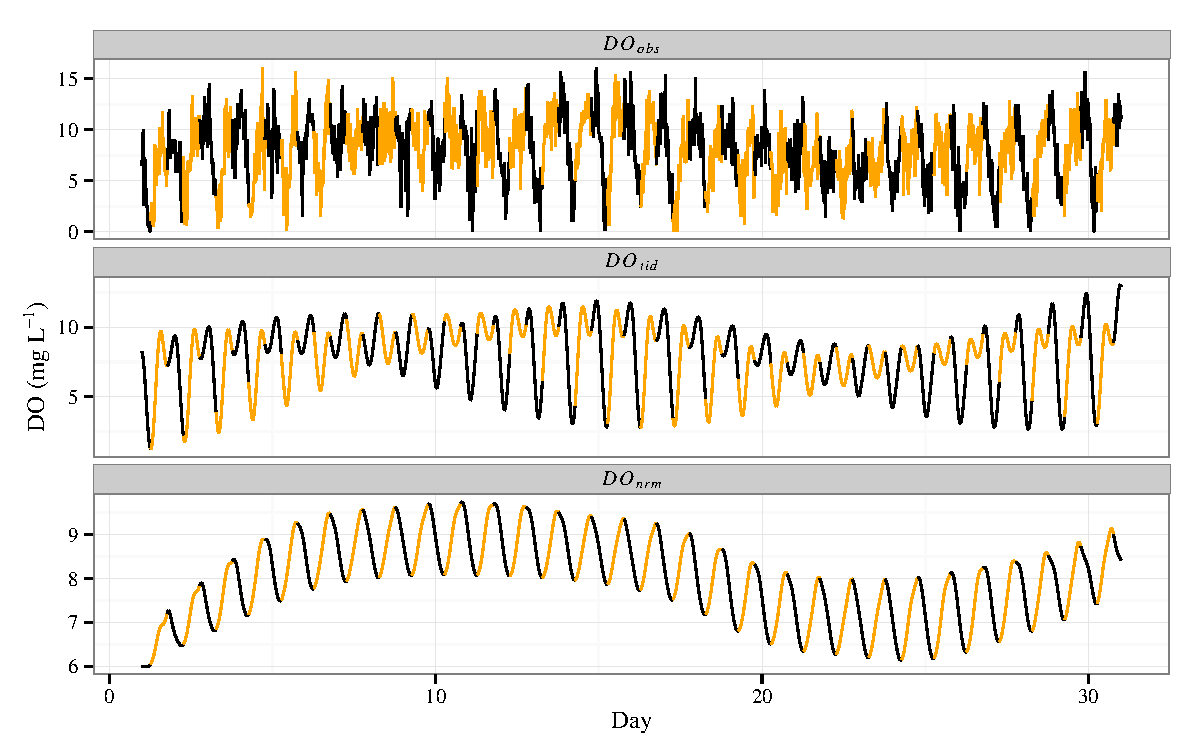
\includegraphics[width=\maxwidth]{figure/do_dtd} 

}

\caption[Example of detiding a simulated \ac{DO} time series]{Example of detiding a simulated \ac{DO} time series.  $DO_{obs}$ represents an additive time series as in \cref{do_obs_all}, $DO_{tid}$ represents the predicted values of \ac{DO} conditional on tidal height and time (\cref{do_tid}), and $DO_{nrm}$ represents the detided values of \ac{DO} conditional on constant tidal height and time (\cref{do_nrm}).  Yellow indicates daylight periods.\label{fig:do_dtd}}
\end{figure}


\end{knitrout}
\vfill
\clearpage

% example of creating simulated time series
\centering\vspace*{\fill}
\begin{knitrout}
\definecolor{shadecolor}{rgb}{0.969, 0.969, 0.969}\color{fgcolor}\begin{figure}[!ht]


{\centering 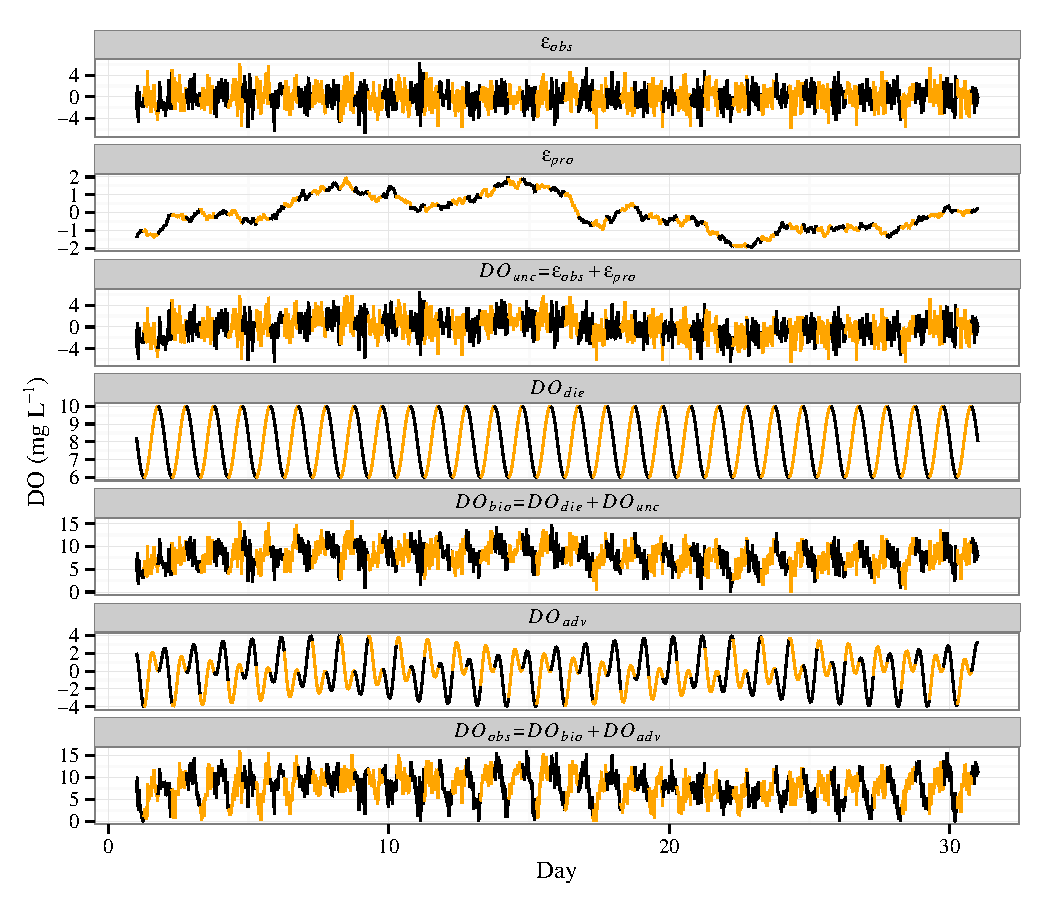
\includegraphics[width=\maxwidth]{figure/do_sim} 

}

\caption[Example of each component of a simulated \ac{DO} time series for testing weighted regression]{Example of each component of a simulated \ac{DO} time series for testing weighted regression.  The time series were created using \cref{do_obs,do_bio,do_unc,do_obs_all,do_sin,do_unc_n,deltdo,deltx,do_advp,do_adv}. Yellow indicates daylight periods.\label{fig:do_sim}}
\end{figure}


\end{knitrout}
\vfill
\clearpage

% plot of representative time series for simulation
\centering\vspace*{\fill}
\begin{knitrout}
\definecolor{shadecolor}{rgb}{0.969, 0.969, 0.969}\color{fgcolor}\begin{figure}[!ht]


{\centering 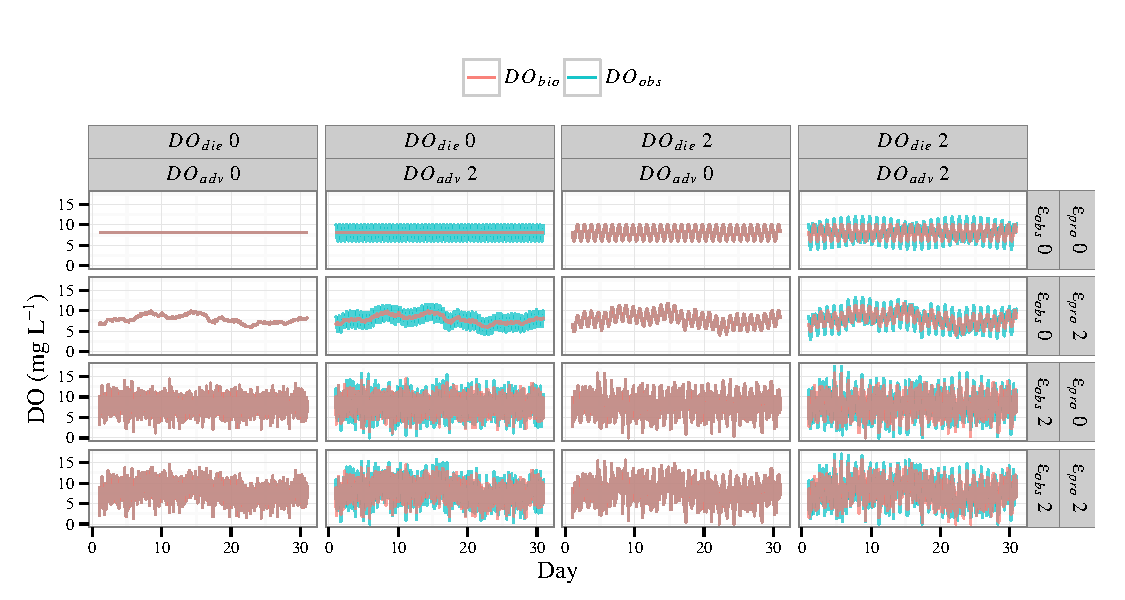
\includegraphics[width=\textwidth]{figure/sim_ex} 

}

\caption[Representative examples of simulated time series of observed \ac{DO} ($DO_{obs}$) and biological \ac{DO} ($DO_{bio}$, as a component of observed) created by varying each of four parameters]{Representative examples of simulated time series of observed \ac{DO} ($DO_{obs}$) and biological \ac{DO} ($DO_{bio}$, as a component of observed) created by varying each of four parameters: strength of tidal association with \ac{DO} signal ($DO_{adv}$), amount of process uncertainty ($\epsilon_{pro}$), amount of observation observation uncertainty ($\epsilon_{obs}$), and strength of diel \ac{DO} component ($DO_{die}$).  Parameter values represent the minimum and maximum used in the simulations as mg L$^{-1}$ of \ac{DO}.\label{fig:sim_ex}}
\end{figure}


\end{knitrout}
\vfill
\clearpage

% example of error surfaces 
\centering\vspace*{\fill}
\begin{knitrout}
\definecolor{shadecolor}{rgb}{0.969, 0.969, 0.969}\color{fgcolor}\begin{figure}[!ht]


{\centering 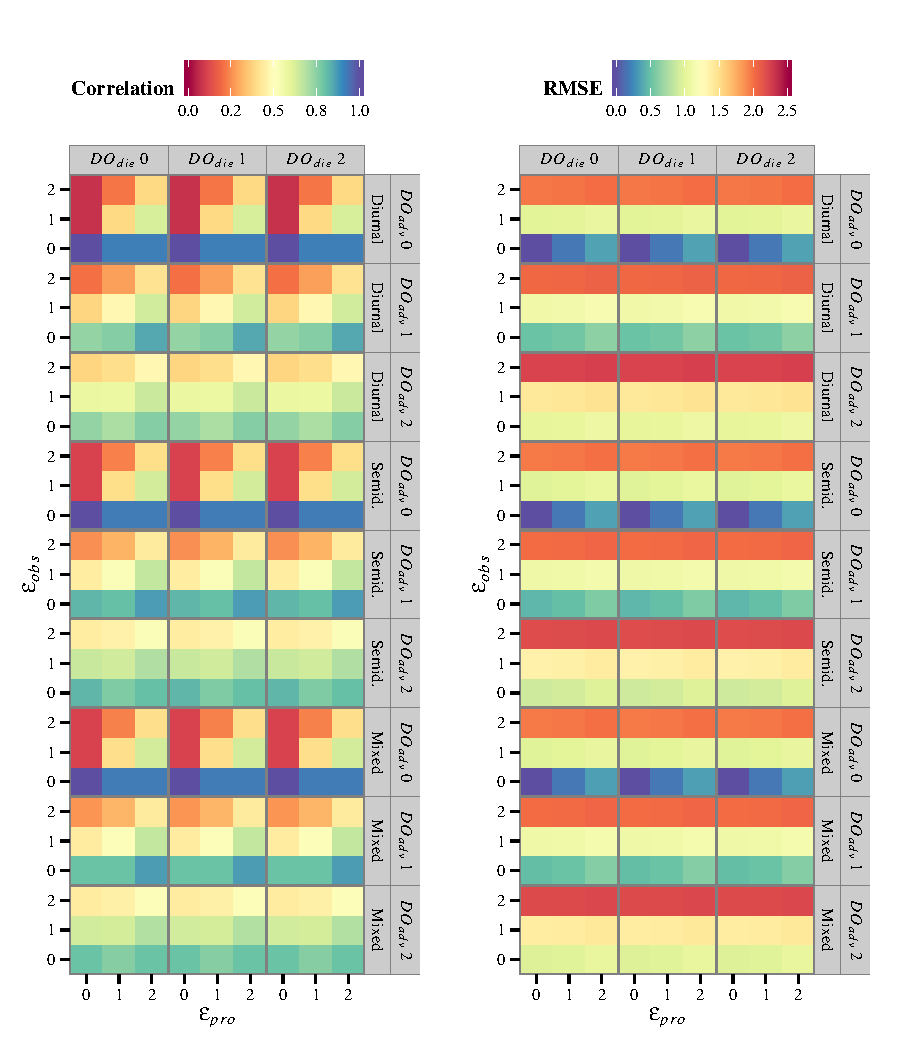
\includegraphics[width=\maxwidth]{figure/err_surf1} 

}

\caption[Correlations and errors (\ac{RMSE}) for detided \ac{DO} time series ($DO_{dtd}$) from weighted regression with `true' biological \ac{DO} ($DO_{bio}$) for varying simulation parameters]{Correlations and errors (\ac{RMSE}) for detided \ac{DO} time series ($DO_{dtd}$) from weighted regression with `true' biological \ac{DO} ($DO_{bio}$) for varying simulation parameters: strength of tidal association with \ac{DO} signal ($DO_{adv}$), amount of process uncertainty ($\epsilon_{pro}$), amount of observation observation uncertainty ($\epsilon_{obs}$), and strength of diel \ac{DO} component ($DO_{die}$).  Each tile represents the correlation or error from results for a given combination of simulation parameters averaged for all window widths (\cref{fig:err_surf2}).\label{fig:err_surf1}}
\end{figure}


\end{knitrout}
\vfill
\clearpage

% example of error surfaces 
\centering\vspace*{\fill}
\begin{knitrout}
\definecolor{shadecolor}{rgb}{0.969, 0.969, 0.969}\color{fgcolor}\begin{figure}[!ht]


{\centering 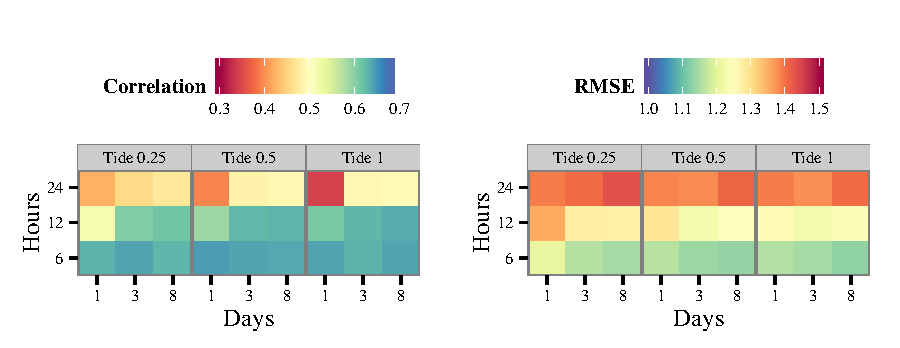
\includegraphics[width=\maxwidth]{figure/err_surf2} 

}

\caption[Correlations and errors (\ac{RMSE}) for detided \ac{DO} time series ($DO_{dtd}$) from weighted regression with `true' biological \ac{DO} ($DO_{bio}$) for varying half window widths]{Correlations and errors (\ac{RMSE}) for detided \ac{DO} time series ($DO_{dtd}$) from weighted regression with `true' biological \ac{DO} ($DO_{bio}$) for varying half window widths: days, hour of day, and proportion of tidal range.  Each tile represents the correlation or error from results for a given combination of window widths averaged for all simulation parameters (\cref{fig:err_surf2}).\label{fig:err_surf2}}
\end{figure}


\end{knitrout}
\vfill
\clearpage

% maps of each case
\centering\vspace*{\fill}
\begin{knitrout}
\definecolor{shadecolor}{rgb}{0.969, 0.969, 0.969}\color{fgcolor}\begin{figure}[!ht]


{\centering 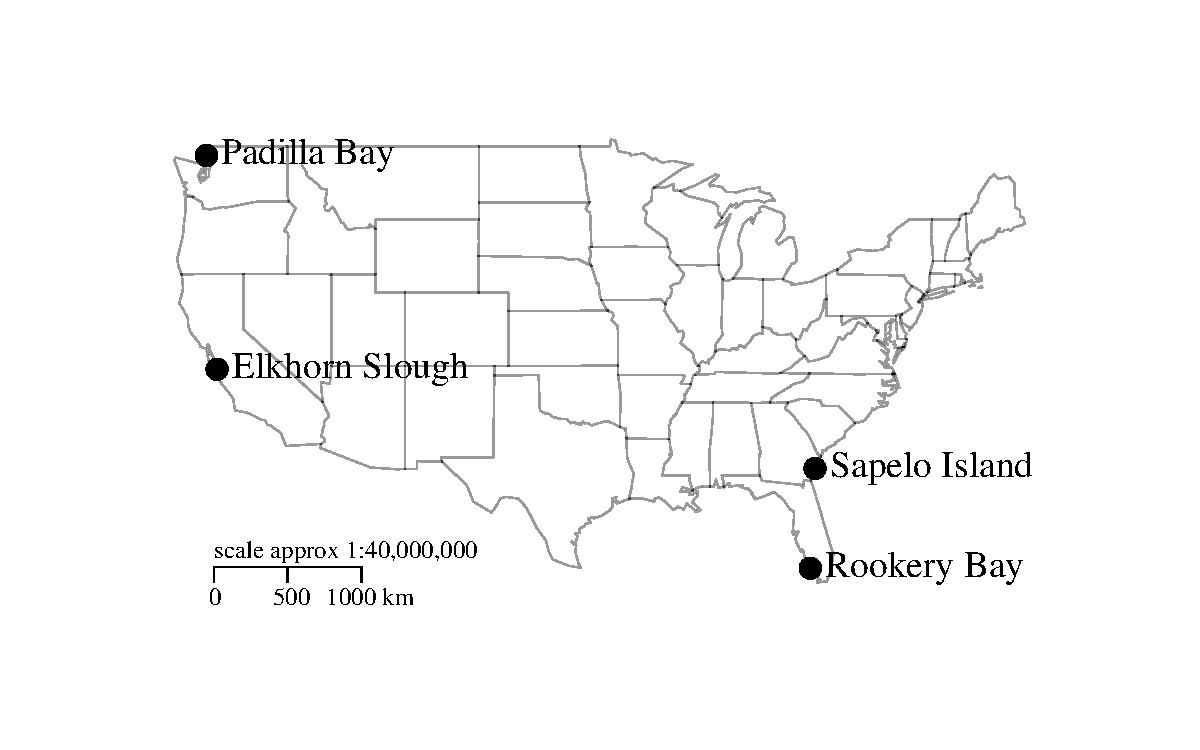
\includegraphics[width=\maxwidth]{figure/case_map} 

}

\caption[Locations of \ac{NERRS} sites used as case studies to validate weighted regression]{Locations of \ac{NERRS} sites used as case studies to validate weighted regression.  Stations at each reserve are ELKVM (Vierra Mouth at Elkhorn Slough), PDBBY (Bayview Channel at Padilla Bay), RKBMB (Middle Blackwater River at Rookery Bay), and SAPDC (Dean Creek at Sapelo Island).\label{fig:case_map}}
\end{figure}


\end{knitrout}
\vfill
\clearpage

% example from SAPHD, phase out
\centering\vspace*{\fill}
\begin{knitrout}
\definecolor{shadecolor}{rgb}{0.969, 0.969, 0.969}\color{fgcolor}\begin{figure}[!ht]


{\centering 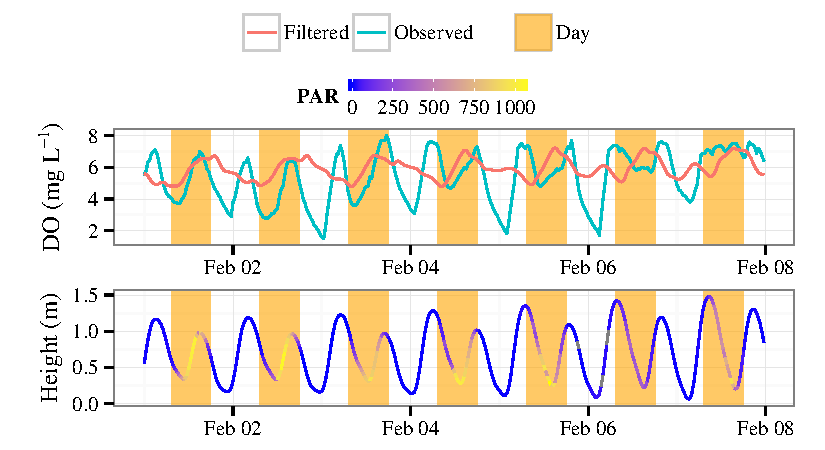
\includegraphics[width=0.8\textwidth]{figure/phase_out} 

}

\caption[Continuous \ac{DO} time series before (observed) and after (detided) detiding with weighted regression (top) and tidal height colored by total photosynthetically active radiation (bottom, mmol m$^{-2}$)]{Continuous \ac{DO} time series before (observed) and after (detided) detiding with weighted regression (top) and tidal height colored by total photosynthetically active radiation (bottom, mmol m$^{-2}$). Results are for the Sapelo Island station for a seven day period when high tide events were out of phase with diel periods, creating lower than expected observed \ac{DO} during night and day periods. Detided values are based on a weighted regression with half window widths of six days, one hour within each day, and tidal height proportion of one half.\label{fig:phase_out}}
\end{figure}


\end{knitrout}
\vfill
\clearpage

% example from SAPHD, phase in
\centering\vspace*{\fill}
\begin{knitrout}
\definecolor{shadecolor}{rgb}{0.969, 0.969, 0.969}\color{fgcolor}\begin{figure}[!ht]


{\centering 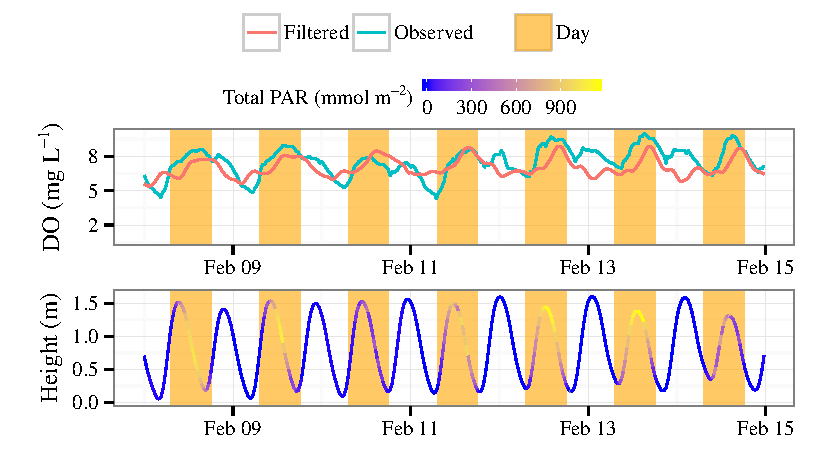
\includegraphics[width=0.8\textwidth]{figure/phase_in} 

}

\caption[Continuous \ac{DO} time series before (observed) and after (detided) detiding with weighted regression (top) and tidal height colored by total photosynthetically active radiation (bottom, mmol m$^{-2}$)]{Continuous \ac{DO} time series before (observed) and after (detided) detiding with weighted regression (top) and tidal height colored by total photosynthetically active radiation (bottom, mmol m$^{-2}$). Results are for the Sapelo Island station for a seven day period when high tide events were in phase with diel periods, creating higher than expected observed \ac{DO} during night and day periods. Detided values are based on a weighted regression with half window widths of six days, one hour within each day, and tidal height proportion of one half.\label{fig:phase_in}}
\end{figure}


\end{knitrout}
\vfill
\clearpage

% example from SAPDC
\centering\vspace*{\fill}
\begin{knitrout}
\definecolor{shadecolor}{rgb}{0.969, 0.969, 0.969}\color{fgcolor}\begin{figure}[!ht]


{\centering 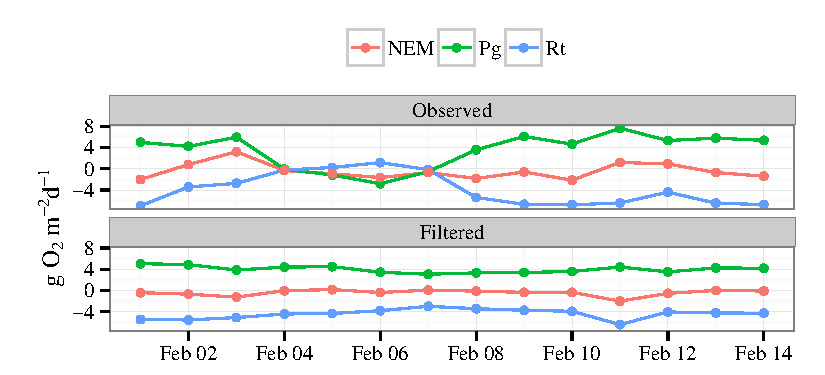
\includegraphics[width=0.8\textwidth]{figure/case_ex} 

}

\caption[Example of daily mean metabolism (net ecosystem metabolism, gross production, and total respiration) before (observed) and after (detided) detiding with weighted regression]{Example of daily mean metabolism (net ecosystem metabolism, gross production, and total respiration) before (observed) and after (detided) detiding with weighted regression. Results are for the Sapelo Island station for a two week period in February, 2012 when high tide was out of phase with the diel cycle during the first week (\cref{fig:phase_out}) and in phase during the second week (\cref{fig:phase_in}).\label{fig:case_ex}}
\end{figure}


\end{knitrout}

% plots of summarized metabolism estimates, before/after detiding
% ELKVM, PDBBY
\centering\vspace*{\fill}
\begin{knitrout}
\definecolor{shadecolor}{rgb}{0.969, 0.969, 0.969}\color{fgcolor}\begin{figure}[!ht]


{\centering 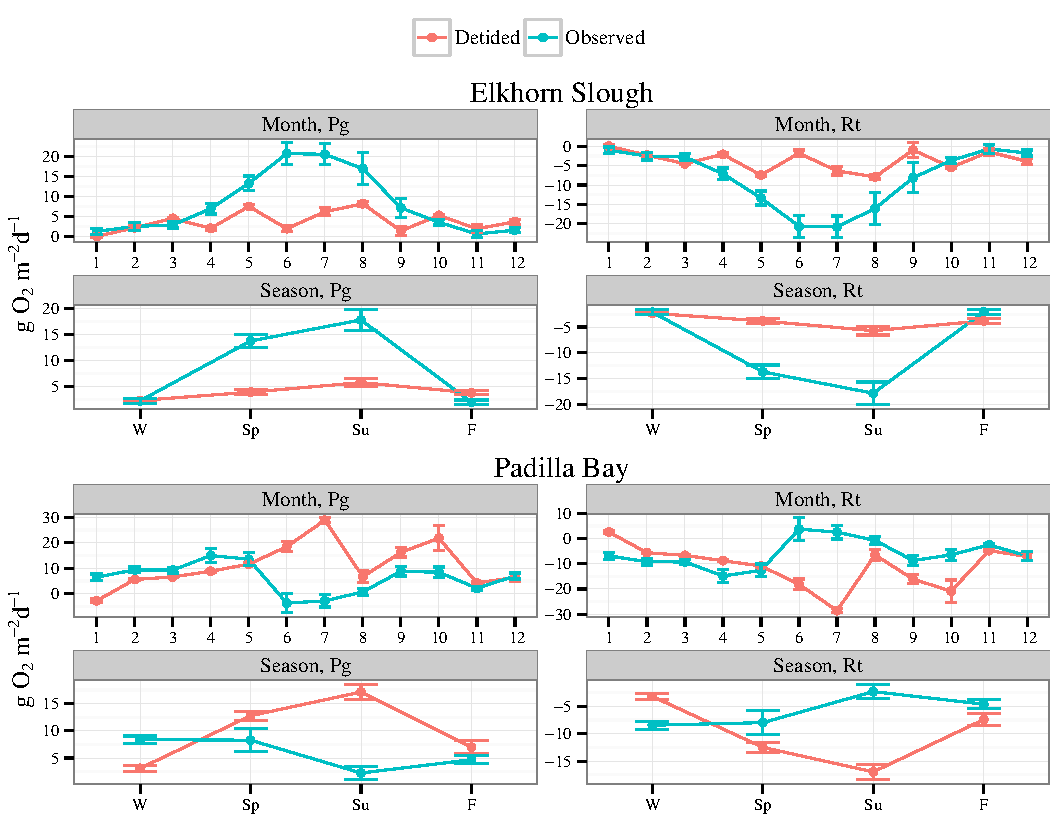
\includegraphics[width=\maxwidth]{figure/metab_sum1} 

}

\caption[Means and standard errors of daily metabolism estimates (gross production, total respiration) aggregated by month and season]{Means and standard errors of daily metabolism estimates (gross production, total respiration) aggregated by month and season.  Aggregated estimates are for Elkhorn Slough and Padilla Bay from observed and detided \ac{DO} time series.\label{fig:metab_sum1}}
\end{figure}


\end{knitrout}
\vfill
\clearpage

% RKBMB, SAPDC
% plots of summarized metabolism estimates, before/after detiding
\centering\vspace*{\fill}
\begin{knitrout}
\definecolor{shadecolor}{rgb}{0.969, 0.969, 0.969}\color{fgcolor}\begin{figure}[!ht]


{\centering 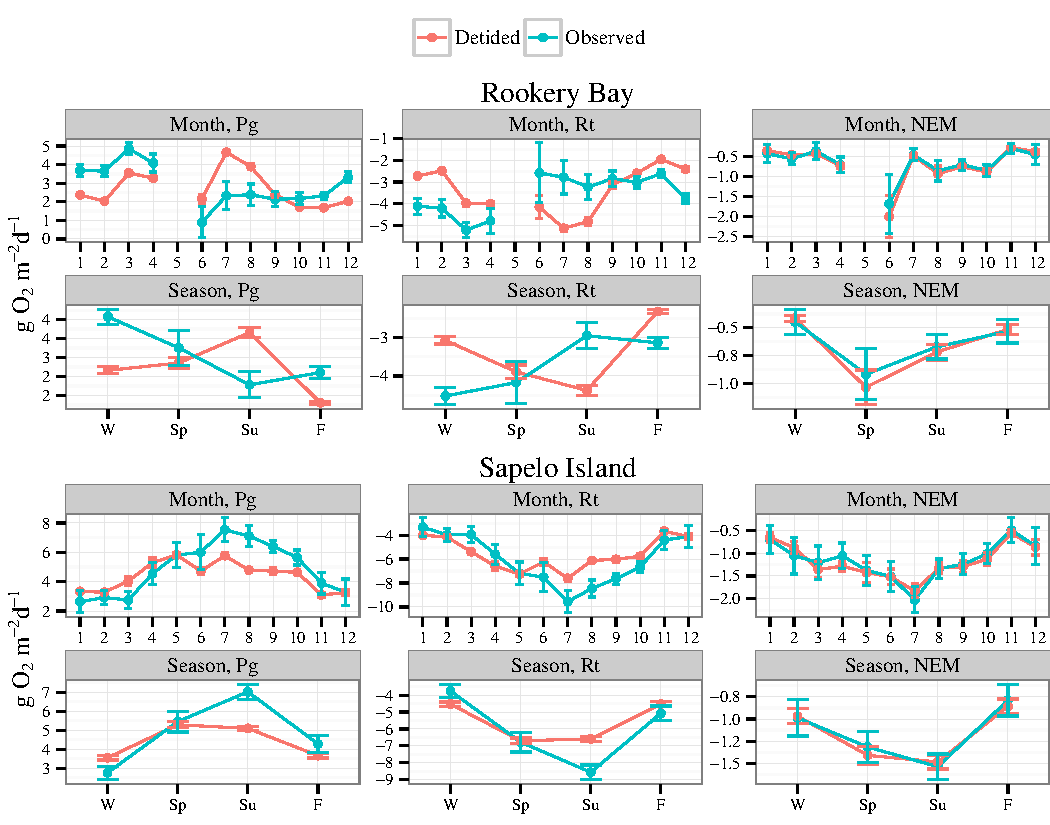
\includegraphics[width=\maxwidth]{figure/metab_sum2} 

}

\caption[Means and standard errors of daily metabolism estimates (gross production, total respiration) aggregated by month and season]{Means and standard errors of daily metabolism estimates (gross production, total respiration) aggregated by month and season.  Aggregated estimates are for Rookery Bay and Sapelo Island from observed and detided \ac{DO} time series.  May was removed from Rookery Bay because of incomplete data.\label{fig:metab_sum2}}
\end{figure}


\end{knitrout}
\vfill
\clearpage

%%%%%%
% tables

\section{Tables}

% summary of simulation performance for detided and biological, sim parameters
% latex.default(tab, file = "", where = "h", rowlabel = "Parameter",      caption = cap.val, caption.loc = "top", rgroup = Parms, n.rgroup = rep(3,          4), cgroup = c("Correlation", "RMSE"), n.cgroup = c(5,          5), rowname = rows, colheads = rep(c("Min", "25\\textsuperscript{th}",          "Mean", "75\\textsuperscript{th}", "Max"), 2), label = "tab:dtd_perf1") 
%
\begin{table}[h]
\caption{Summary (range, mean, percentiles) of correlations and error estimates comparing detided and biological \ac{DO} time series for different simulation parameters ($DO_{die}$, $DO_{adv}$, $\epsilon_{pro}$, $\epsilon_{obs}$).  Values represent averages from multiple simulations with common parameters (e.g., row one is a summary of all simulations for which diel \ac{DO} component was zero).\label{tab:dtd_perf1}} 
\begin{center}
\begin{tabular}{llllllclllll}
\hline\hline
\multicolumn{1}{l}{\bfseries Parameter}&\multicolumn{5}{c}{\bfseries Correlation}&\multicolumn{1}{c}{\bfseries }&\multicolumn{5}{c}{\bfseries RMSE}\tabularnewline
\cline{2-6} \cline{8-12}
\multicolumn{1}{l}{}&\multicolumn{1}{c}{Min}&\multicolumn{1}{c}{25\textsuperscript{th}}&\multicolumn{1}{c}{Mean}&\multicolumn{1}{c}{75\textsuperscript{th}}&\multicolumn{1}{c}{Max}&\multicolumn{1}{c}{}&\multicolumn{1}{c}{Min}&\multicolumn{1}{c}{25\textsuperscript{th}}&\multicolumn{1}{c}{Mean}&\multicolumn{1}{c}{75\textsuperscript{th}}&\multicolumn{1}{c}{Max}\tabularnewline
\hline
{\bfseries $\boldsymbol{DO_{die}}$}&&&&&&&&&&&\tabularnewline
~~0&-0.78&0.30&0.53&0.82&1.00&&0.00&0.68&1.22&1.97&2.39\tabularnewline
~~1&-0.28&0.38&0.61&0.88&1.00&&0.00&0.59&1.20&1.96&2.40\tabularnewline
~~2&-0.39&0.46&0.65&0.90&1.00&&0.00&0.62&1.22&1.97&2.40\tabularnewline
\hline
{\bfseries $\boldsymbol{DO_{adv}}$}&&&&&&&&&&&\tabularnewline
~~0& 0.00&0.27&0.57&0.93&1.00&&0.00&0.34&1.07&1.96&2.12\tabularnewline
~~1&-0.78&0.37&0.59&0.83&1.00&&0.00&0.63&1.18&1.98&2.12\tabularnewline
~~2&-0.78&0.47&0.63&0.82&1.00&&0.00&0.98&1.38&1.99&2.40\tabularnewline
\hline
{\bfseries $\boldsymbol{\epsilon_{pro}}$}&&&&&&&&&&&\tabularnewline
~~0&-0.78&0.34&0.58&0.86&1.00&&0.00&0.63&1.19&1.96&2.40\tabularnewline
~~1&-0.78&0.37&0.59&0.85&1.00&&0.00&0.63&1.21&1.97&2.40\tabularnewline
~~2&-0.78&0.41&0.61&0.85&1.00&&0.00&0.63&1.24&1.98&2.40\tabularnewline
\hline
{\bfseries $\boldsymbol{\epsilon_{obs}}$}&&&&&&&&&&&\tabularnewline
~~0&-0.78&0.31&0.65&0.98&1.00&&0.00&0.29&0.92&1.50&2.40\tabularnewline
~~1& 0.05&0.37&0.57&0.81&0.99&&0.07&0.98&1.18&1.49&2.39\tabularnewline
~~2& 0.05&0.40&0.57&0.70&0.99&&0.15&1.06&1.54&2.01&2.40\tabularnewline
\hline
\end{tabular}
\end{center}
\end{table}



% summary of simulation performance for detided and biological, window widths
% latex.default(tab, file = "", rowlabel = "Window", caption = cap.val,      caption.loc = "top", rgroup = Parms, n.rgroup = rep(3, 3),      cgroup = c("Correlation", "RMSE"), n.cgroup = c(5, 5), rowname = rows,      colheads = rep(c("Min", "25\\textsuperscript{th}", "Mean",          "75\\textsuperscript{th}", "Max"), 2), label = "tab:dtd_perf2") 
%
\begin{table}[!tbp]
\caption{Summary (range, mean, percentiles) of correlations and error estimates comparing detided and biological \ac{DO} time series for simulations using different half window widths in the weighted regressions (days, hours, and proportion of tidal range).  Values represent averages from multiple simulations with common window values (e.g., row one is a summary of all simulations for which the half window width was one day).\label{tab:dtd_perf2}} 
\begin{center}
\begin{tabular}{llllllclllll}
\hline\hline
\multicolumn{1}{l}{\bfseries Window}&\multicolumn{5}{c}{\bfseries Correlation}&\multicolumn{1}{c}{\bfseries }&\multicolumn{5}{c}{\bfseries RMSE}\tabularnewline
\cline{2-6} \cline{8-12}
\multicolumn{1}{l}{}&\multicolumn{1}{c}{Min}&\multicolumn{1}{c}{25\textsuperscript{th}}&\multicolumn{1}{c}{Mean}&\multicolumn{1}{c}{75\textsuperscript{th}}&\multicolumn{1}{c}{Max}&\multicolumn{1}{c}{}&\multicolumn{1}{c}{Min}&\multicolumn{1}{c}{25\textsuperscript{th}}&\multicolumn{1}{c}{Mean}&\multicolumn{1}{c}{75\textsuperscript{th}}&\multicolumn{1}{c}{Max}\tabularnewline
\hline
{\bfseries Days}&&&&&&&&&&&\tabularnewline
~~1&-0.78&0.63&0.78&0.97&1.00&&0.00&0.28&0.74&1.04&2.12\tabularnewline
~~3&-0.07&0.40&0.56&0.75&1.00&&0.00&0.99&1.15&1.28&2.08\tabularnewline
~~6& 0.00&0.26&0.45&0.58&1.00&&0.00&1.95&1.75&2.05&2.40\tabularnewline
\hline
{\bfseries Hours}&&&&&&&&&&&\tabularnewline
~~1&-0.78&0.36&0.57&0.82&1.00&&0.00&0.63&1.22&1.96&2.40\tabularnewline
~~3& 0.00&0.40&0.61&0.87&1.00&&0.00&0.58&1.20&1.97&2.36\tabularnewline
~~6& 0.03&0.37&0.61&0.85&1.00&&0.00&0.64&1.22&1.98&2.40\tabularnewline
\hline
{\bfseries Tide}&&&&&&&&&&&\tabularnewline
~~0.25& 0.00&0.42&0.64&0.91&1.00&&0.00&0.51&1.14&1.97&2.21\tabularnewline
~~0.5& 0.06&0.43&0.63&0.88&1.00&&0.00&0.61&1.20&1.97&2.27\tabularnewline
~~1&-0.78&0.30&0.52&0.79&1.00&&0.00&0.73&1.30&1.97&2.40\tabularnewline
\hline
\end{tabular}
\end{center}
\end{table}



% descriptive table of case studies
% latex.default(tab, file = "", rowlabel = "Site", insert.bottom = foot.val,      caption = cap.val, caption.loc = "top", cgroup = c("Tidal amplitude",          "Water quality", "Metabolism\\textsuperscript{\\textit{a}}"),      n.cgroup = c(4, 4, 3), rowname = rows, colheads = c("O1",          "P1", "M2", "S2", "DO", "Chl", "Sal", "Temp", "Pg", "Rt",          "NEM"), label = "tab:case_att") 
%
\begin{table}[!tbp]
\caption{Summary statistics of tidal component amplitudes (m), selected water quality parameters (\ac{DO} mg L$^{-1}$, chlorophyll-a $\mu$g L$^{-1}$, salinity psu, water temperature $^{\circ}$C)  and metabolism estimates (gross production, respiration, and net ecosystem metabolism as g m$^{-2}$ d$^{-1}$) for each case study.  Tidal components are principal lunar semidiurnal (O1, frequency 25.82 hours), solar diurnal (P1, 24.07 hours), lunar semidiurnal (M2, 12.42 hours), and solar semidiurnal (S2, 12 hours) estimated from harmonic regressions of tidal height (\texttt{oce} package in R, \citealt{Foreman89}, \citetalias{RDCT14}).  Water quality data are averages for the entire period of record (30 minute observations) for each site.  Metabolism estimates are means of daily integrated values.\label{tab:case_att}} 
\begin{center}
\begin{tabular}{lllllcllllclll}
\hline\hline
\multicolumn{1}{l}{\bfseries Site}&\multicolumn{4}{c}{\bfseries Tidal amplitude}&\multicolumn{1}{c}{\bfseries }&\multicolumn{4}{c}{\bfseries Water quality}&\multicolumn{1}{c}{\bfseries }&\multicolumn{3}{c}{\bfseries Metabolism\textsuperscript{\textit{a}}}\tabularnewline
\cline{2-5} \cline{7-10} \cline{12-14}
\multicolumn{1}{l}{}&\multicolumn{1}{c}{O1}&\multicolumn{1}{c}{P1}&\multicolumn{1}{c}{M2}&\multicolumn{1}{c}{S2}&\multicolumn{1}{c}{}&\multicolumn{1}{c}{DO}&\multicolumn{1}{c}{Chl}&\multicolumn{1}{c}{Sal}&\multicolumn{1}{c}{Temp}&\multicolumn{1}{c}{}&\multicolumn{1}{c}{Pg}&\multicolumn{1}{c}{Rt}&\multicolumn{1}{c}{NEM}\tabularnewline
\hline
ELKVM&0.24&0.12&0.48&0.13&&7.87&3.87&32.43&13.78&&8.14&-8.19&-0.05\tabularnewline
PDBBY&0.46&0.23&0.63&0.15&&8.97&2.24&29.17&10.44&&5.95&-5.90& 0.05\tabularnewline
RKBMB&0.13&0.04&0.36&0.10&&4.48&4.50&30.53&25.85&&3.02&-3.62&-0.60\tabularnewline
SAPDC&0.10&0.02&0.54&0.07&&4.96&5.98&27.30&21.77&&4.89&-6.04&-1.16\tabularnewline
\hline
\end{tabular}
\end{center}
\footnotesize\textsuperscript{\textit{a}}Pg: gross production, Rt: respiration, NEM: net ecosystem metabolism\end{table}



% correlations with tide before/after wtreg
% latex.default(tab, file = "", rowlabel = "Site", rgroup = unique(rows),      n.rgroup = rep(2, 4), insert.bottom = foot.val, caption = cap.val,      colheads = c("DO", "Pg\\textsuperscript{\\textit{a}}", "Rt",          "NEM"), caption.loc = "top", rowname = rep(c("Observed",          "Detided"), 4), label = "tab:cor_res") 
%
\begin{table}[!tbp]
\caption{Correlations of tidal changes at each site with continuous \ac{DO} observations and metabolism estimates (gross production, respiration, and net metabolism) before (observed) and after (detided) detiding with weighted regression.  \ac{DO} values are correlated with predicted tidal height at each observation, whereas metabolism estimates are correlated with mean tidal height change between observations during day, night, or total day periods for production, respiration, and net metabolism, respectively.\label{tab:cor_res}} 
\begin{center}
\begin{tabular}{lllll}
\hline\hline
\multicolumn{1}{l}{Site}&\multicolumn{1}{c}{DO}&\multicolumn{1}{c}{Pg\textsuperscript{\textit{a}}}&\multicolumn{1}{c}{Rt}&\multicolumn{1}{c}{NEM}\tabularnewline
\hline
{\bfseries ELKVM}&&&&\tabularnewline
~~Observed& 0.47***& 0.60***& 0.73***& 0.35***\tabularnewline
~~Detided& 0.02*& 0.19***& 0.13*& 0.06 \tabularnewline
\hline
{\bfseries PDBBY}&&&&\tabularnewline
~~Observed&-0.45***&-0.33***&-0.46***&-0.25***\tabularnewline
~~Detided& 0.07***& 0.48***& 0.47***&-0.21***\tabularnewline
\hline
{\bfseries RKBMB}&&&&\tabularnewline
~~Observed& 0.28***& 0.34***& 0.39***& 0.24***\tabularnewline
~~Detided&-0.02**&-0.31***&-0.36***& 0.12*\tabularnewline
\hline
{\bfseries SAPDC}&&&&\tabularnewline
~~Observed& 0.48***& 0.54***& 0.71***& 0.41***\tabularnewline
~~Detided&-0.03***& 0.16**& 0.18***&-0.05 \tabularnewline
\hline
\end{tabular}
\end{center}
\footnotesize *$p<0.05$; **$p<0.01$; ***$p<0.001$\\\textsuperscript{\textit{a}}Pg: gross production, Rt: respiration, NEM: net ecosystem metabolism\end{table}



% case study metabolism results, including perc anom
% latex.default(tab, file = "", rowlabel = "Site", insert.bottom = foot.val,      caption = cap.val, caption.loc = "top", rgroup = unique(to_tab$Site),      n.rgroup = rep(2, 4), cgroup = c("Pg\\textsuperscript{\\textit{a}}",          "Rt", "NEM"), n.cgroup = c(3, 3, 2), rowname = rows,      colheads = c(rep(c("Mean", "Std. Err.", "Anom"), 2), c("Mean",          "Std. Err.")), label = "tab:case_res") 
%
\begin{table}[!tbp]
\caption{Summary of metabolism estimates (gross production, respiration, and net metabolism) for case studies using \ac{DO} time series before (observed) and after (detided) detiding with weighted regression.  Means and standard errors are based on daily integrated metabolism estimates.  Anomalous values are the proportion of metabolism estimates that were negative for gross production and positive for respiration.  Results are for weighted regressions with half window widths of six days, one hour within each day, and a tidal height proportion of one half.\label{tab:case_res}} 
\begin{center}
\begin{tabular}{llllclllcll}
\hline\hline
\multicolumn{1}{l}{\bfseries Site}&\multicolumn{3}{c}{\bfseries Pg\textsuperscript{\textit{a}}}&\multicolumn{1}{c}{\bfseries }&\multicolumn{3}{c}{\bfseries Rt}&\multicolumn{1}{c}{\bfseries }&\multicolumn{2}{c}{\bfseries NEM}\tabularnewline
\cline{2-4} \cline{6-8} \cline{10-11}
\multicolumn{1}{l}{}&\multicolumn{1}{c}{Mean}&\multicolumn{1}{c}{Std. Err.}&\multicolumn{1}{c}{Anom}&\multicolumn{1}{c}{}&\multicolumn{1}{c}{Mean}&\multicolumn{1}{c}{Std. Err.}&\multicolumn{1}{c}{Anom}&\multicolumn{1}{c}{}&\multicolumn{1}{c}{Mean}&\multicolumn{1}{c}{Std. Err.}\tabularnewline
\hline
{\bfseries ELKVM}&&&&&&&&&&\tabularnewline
~~Observed& 8.14&0.67&0.19&& -8.19&0.69&0.21&&-0.05&0.16\tabularnewline
~~Detided& 3.63&0.23&0.17&& -3.67&0.24&0.17&&-0.04&0.05\tabularnewline
\hline
{\bfseries PDBBY}&&&&&&&&&&\tabularnewline
~~Observed& 5.95&0.69&0.22&& -5.90&0.74&0.19&& 0.05&0.22\tabularnewline
~~Detided&10.36&0.63&0.13&&-10.32&0.63&0.13&& 0.04&0.08\tabularnewline
\hline
{\bfseries RKBMB}&&&&&&&&&&\tabularnewline
~~Observed& 3.02&0.14&0.09&& -3.62&0.15&0.08&&-0.60&0.06\tabularnewline
~~Detided& 3.73&0.09&0.01&& -4.35&0.10&0.00&&-0.62&0.04\tabularnewline
\hline
{\bfseries SAPDC}&&&&&&&&&&\tabularnewline
~~Observed& 4.89&0.23&0.13&& -6.04&0.25&0.11&&-1.16&0.09\tabularnewline
~~Detided& 4.85&0.08&0.00&& -6.04&0.10&0.00&&-1.19&0.05\tabularnewline
\hline
\end{tabular}
\end{center}
\textsuperscript{\textit{a}}Pg: gross production, Rt: respiration, NEM: net ecosystem metabolism\end{table}


\clearpage

%%%%%%
% multimedia files, appendices

\raggedbottom
\raggedright
\setlength{\parindent}{0.5in}

\section{Multimedia} \label{multi}
The supporting information for this manuscript includes a graphical illustration of the weighting scheme described in the material and procedures section (\href{http://spark.rstudio.com/beckmw/weights_widget}{http://spark.rstudio.com/beckmw/weights\_widget}), results for each simulation (\href{http://spark.rstudio.com/beckmw/detiding_sims}{http://spark.rstudio.com/beckmw/detiding\_sims}), and results for each case study (\href{http://spark.rstudio.com/beckmw/detiding_cases}{http://spark.rstudio.com/beckmw/detiding\_cases}).  Each link is a graphical summary of data based on interactive inputs to support the results in the manuscript.

A simple R package with a sample dataset and code to implement weighted regression is also available on GitHub.  Functions are also availabe to estimate ecosystem metabolism.  See the README file on the web page for download instructions and examples: \href{https://github.com/fawda123/WtRegDO}{https://github.com/fawda123/WtRegDO}

\end{document}
